\chapter{General discussion, future work and conclusions}
\label{ch:conc}
\acresetall

%Discovery-driven or observation-driven vs hypothesis driven
%Antarctic lakes are exceptional ecosystems that contain microbial life adapted to extreme polar conditions and the local lake geochemistry.
Metagenomics has proven to be an effective way to map the diversity of Antarctic lake ecosystems and provide hints of how they work.
In combination with metaproteomics and abiotic parameters, in-depth descriptions of the ecosystem functions of Ace Lake and Organic Lake were achieved.
The most noteworthy contribution of these studies has been to describe taxa and microbial processes previously unknown to occur in these lakes, and from these descriptions, generate testable hypotheses of population and ecosystem level function.

\section{Summary of outcomes from this work}
%This has necessitated the development of new ways to extract biological inferences from complex datasets.
The overall objective of this thesis was to study Antarctic lake ecosystems using an integrative metagenomics-driven approach.
In order to do this, methods were developed in chapter \ref{ch:ace} to measure properties of the community that would work alongside metagenomic sequencing to piece together a comprehensive description of ecosystem structure and function.
An epifluorescene microscopy protocol was designed that makes use of 0.01 \textmu{}m pore-size \ac{PCTE} membrane filters.
Using this protocol, cells and \acp{VLP} were successfully visualised and enumerated along the depth profile of Ace Lake, and subsequently in Organic Lake.
The need to develop this method was due to the discontinuation of supply of Anodisc filters, which are the standard filter used for direct counts of \acp{VLP} by epifluorescence microscopy.
Although cell and \ac{VLP} densities are fairly basic properties of the community, their measurement nonetheless revealed surprising results, such as the lack of correspondence between turbidity and cell density in Organic Lake.

A bioinformatic pipeline for analysis of metaproteomic mass spectra was also developed in chapter \ref{ch:ace} that incorporated use of matching metagenomic databases for protein identification and spectral counting to estimate protein abundances.
When applied to the metaproteomic analysis of Ace Lake, this workflow resulted in a greater number of protein identifications than previous work using cross-species matching and showed statistically significant functional differences between the strata of the lake.
It also described the functional capacity of dominant populations in the mixolimnion, particularly transporter use.
The elaboration of a conceptual framework incorporating genomic and functional data in the study Ace Lake laid the groundwork for the subsequent studies on Organic Lake.

In chapter \ref{ch:olv}, two near-complete \ac{OLPV} genomes and a complete \ac{OLV} genome were described.
Genomic analysis of \ac{OLV} indicated it was a new member of the virophage virus family, which obligately utilise a  giant `helper' virus to complete their replication cycle but impair their helper's infectivity in the process.
Comparison of \ac{OLV} and \ac{OLPV} genomes identified shared regions that strongly suggest \ac{OLV} is a virophage of \ac{OLPV}.
The metaproteomic analysis identified both viral capsids confirming members of the population were actively replicating viruses and not, for example, accessory genetic elements.
The availibility of \textsc{DNA} sequences from the whole community meant the most likely host, \emph{Pyramimonas}, could be identified from the \ac{SSU} genes.
The inferred interaction of the \ac{OLV}, \ac{OLPV} and host was used to generate a model of their population dynamics that showed if \ac{OLV} acts as a `predator of a predator', this would lead to increased frequency of population cycling.
This was hypothesized to function in the Antarctic lake ecosystem as means to increase dissolved carbon release and secondary production over the summer season.
Potential relatives of the \ac{OLV} were also found in Ace Lake and other aquatic environments indicating virophage may play an influential role in other ecosystems.

In chapter \ref{ch:org} a profile of the Organic Lake microbial taxonomic composition and potential for nutrient cycling was determined.
The community was found to consist primarily of eucaryotic algae related to \emph{Dunaliella} and three heterotrophic bacterial genera: \emph{Marinobacter}, \emph{Roseovarius} and \emph{Psychroflexus}.
The suboxic bottom zone of Organic Lake additionally contained lower abundance populations of \emph{Firmicutes}, \emph{Deltaproteobacteria} and \emph{Epsilonproteobacteria}.
Examination of genes involved in carbon cycling indicated a net loss of carbon could occur as potential for fixation was lower than for respiration.
However, genes for photo- and lithoheterotrophic pathways linked to the dominant bacterial lineages were abundant; in particular \ac{AAnP} genes were much higher than in any other aquatic environment surveyed.
Use of energy sources apart from organic carbon was hypothesized to be a specific adaptation of the heterotrophic bacterial population to conserve carbon within the system.
The capacity for nitrogen cycling also showed a shift away from fixation and a predominance of recycling of reduced nitrogen compounds.
This was similarly hypothesized to function as a mechanism to limit nitrogen loss.
A targeted search for genes involved in \ac{DMS} conversions found an abundance of \ac{DMSP} lyase genes indicating lysis of \ac{DMSP} is the likely source of the high \ac{DMS} levels that has been detected in Organic Lake.
\ac{DMSP} lyase genes were linked to \emph{Gammaproteobacteria} and \emph{Alphaproteobacteria} indicating \ac{DMSP} is an important carbon and energy source for these bacteria.
Unlike marine environments, \ac{DMSP} lyase genes were more abundant than \ac{DMSP} demethylase genes. 
The only other metagenomes to show comparably high abundance of \ac{DMSP} lyase genes were other hypersaline environments suggesting the DMSP lysis pathway is favoured in high salinity systems. 
%We have used theory to guide our work.

\section{New perspectives and possibilities for future work on Organic Lake}
%The work described in this thesis is part of a program that has pioneering the use of shotgun metagenomics and metaproteomics in Antarctic lakes \cite{Ng2010a, Lauro2011, Yau2011} and the Southern Ocean \cite{Wilkins2012b, Grzymski2012, Williams2012a, Williams2012b}.
To establish a picture of the biotic composition and function of Antarctic lake communities, an observation-driven approach was utilised that allowed for completely new discoveries about these systems to be made.
Bioinformatic pipelines and theoretical models to do this have now been established.
These can be applied to future, similarly observation-based studies of Ace and Organic Lakes to define how they change over time and test our existing models of lake function.
%Some expected outcomes and specifics involved in how these studies could be implemented are described below.
It is also clear that a systems level understanding of the lakes is bolstered by having well-characterised isolates related to members in the community.
Guided by the studies from this thesis, isolation and characterisation of key members of the community, such as \emph{Pyramimonas}, \ac{OLPV}, \ac{OLV}, \emph{Marinobacter} spp. and \emph{Roseovarius} spp. from Organic Lake, could be attempted in the future and may be the only definitive way to test certain hypotheses.
However, other technologies, such as single cell and virus genomics and \ac{SIP}, hold promise for learning about specific populations in the community.
Some experiments that could be used to test specific hypotheses generated by the study of Organic Lake are discussed below, along their expected implications and new perspectives.

\subsection{Organic Lake dynamics over time}
To establish a complete understanding of Organic Lake requires comprehensive descriptions of the microbial community over different time scales.
An obvious next step would be to obtain metagenomic and functional data at other points in the year, particularly the winter, to determine how the microbial community copes with the large seasonal changes in temperature, light and ice-cover.
This can elucidate how the community sustains itself when the absence of light is expected to forestall phototrophic primary production.
%Furthermore, it can determine what stategies phototrophic organisms employ to survive during this period.
\emph{Psychroflexus gondwanensis} in Organic Lake have been shown to peak in abundance during summer demonstrating that certain populations fluctuate seasonally \cite{James1994}.
However, population dynamics over the annual cycle is not well-understood.

Paired metagenomic and metaproteomic analyses of the coastal Southern Ocean have detected dramatic changes between summer and winter bacterioplankton communities \cite{Grzymski2012, Williams2012a}.
Winter samples were dominated by active chemolithoautotrophs including sulphur-oxidising \emph{Gammaproteobacteria} and ammonia oxidising \emph{Crenarcheaota} \cite{Grzymski2012, Williams2012b}.
If the Organic Lake ecosystem reflects that of the coastal Southern Ocean, the small population of chemolithoautotrophic sulphur-oxidising \emph{Proteobacteria} that were detected in the summer could similarly become dominant in the winter.
Succession of the bacterial population by \emph{Crenarchaeota} is not expected to occur as no signatures for \emph{Crenarchaeota} or ammonia oxidation were present in Organic Lake.
Furthermore, if the model proposed for the Organic Lake nitrogen cycle, which avoids oxidised nitrogen forms, holds true, we can expect ammonia oxidising microorganisms will not play a part in the Organic community in the winter unless nitrogen fixation also increases.
%Another possibility is that bacterial populations will simply become dormant over the winter, as seems to occur in Artic sea ice communities \cite{Collins2010}.
In this way, an `-omics' based analysis of Organic Lake community over an annual cycle will shed light on how robust our models of nutrient cycling and concepts of the taxonomic composition are.

Ideally, global analyses would be performed on samples taken over several time points in the year including the transition from ice-covered to melted.
In chapter \ref{ch:olv}, it was evident that between the November and December 2008 samples there was a large change in the viral population in Organic Lake that correlates with melting of the ice-cover.
Samples in the summer spanning the complete transition from ice-covered to thawed would allow organisms and metabolic functions to be related back the effects of the summer melt.
These samples can also be compared back to the 2006 and 2008 samples to establish if there are interannual differences.
Long-term sampling of Southern Ocean coastal surface waters suggests the community is reproducible year by year \cite{Murray2007}.
However, Organic Lake has been shown to be physically variable over a decadal time scale with changes in water level of $\sim$1 m leading to large changes in the water column structure \cite{Gibson1995, Gibson1996}.
Notably, the pycnocline in Organic Lake occurred at 5.7 m in 2008; much lower than 3.5 m where it first reported to occur in 1978 \cite{Franzmann1987b}.
If the lake completely mixes, this would challenge the oxygen-senstitive microbes and processes occurring in the deep zone.
The large physical changes suggests that the microbial community would similarly experience large interannual variability.
Metagenomic sequencing in a future summer season would provide data spanning several years thereby screening the microbial community profile for evidence of a reproducible interannual cycle.

Sampling intensively over a short time scale in the summer will allow us to test the three-species Lotka-Volterra model of the \ac{OLV}, \ac{OLPV} and host algae population.
In the model, the density of each population oscillates in a phase-shifted manner in the sequence: prey, predator and predator of predator.
By observing the natural dynamics of these populations, we can determine if they fit with the proposed model.
If they do fit, the observed population densities can be used to derive the parameters that govern the interaction.
Close observation of these three taxa can suggest if additional modifications to the existing model or alternative models would better fit the data.

\subsection{\acs{OLV} physiology and ecology}
Since the discovery of the \ac{OLV}, two other members of the virophage family have been reported that have afforded a new perspective on \ac{OLV}.
The first of these is the Mavirus (for Maverick virus) so named for its evolutionary relationship with the Maverick/Politon class of eucaryotic transposons \cite{Fischer2011a}.
Like Sputnik, Mavirus has an absolute requirement for a helper virus to replicate, in this case \ac{CroV}, and is deleterious to its helper \cite{Fischer2011a}.
The other virophage reported was called Sputnik 2 (its genome is virtually identical to Sputnik), but unlike Sputnik, it was found both as a separate genome and integrated in its helper, lentille virus \cite{Desnues2012}.
These two virophage systems in culture are associated with heterophic protists making the \ac{OLV} genomic sequence the only data currently available for virophage affecting cosmopolitan phytoplankton species.
Therefore isolating \ac{OLV}, acquiring genomes of \ac{OLV} relatives and determining fundamental properties of \ac{OLV} physiology and dynamics would contribute immensely to our understanding of its role in Organic Lake bringing with it insight into other aquatic systems.

The evidence that Mavirus has the same `virophage' phenotype as Sputnik strengthens the inference that \ac{OLV} does as well.
This is in part because Mavirus and \ac{CroV} and quite divergent from Sputnik and mimivirus respectively, yet retain the same traits \cite{Fischer2010, Fischer2011a}, suggesting the detrimental effect of virophages to their helpers is common to the whole lineage.
These cultured virophages also offer a mechanistic explanation for this to be the case.
As both mimivirus and \ac{CroV} encode much of their transcriptional machinery including all \textsc{RNA} polymerase subunits, they do not need to localise to the nucleus during infection but generate the viral factory in the cytoplasm of their host \cite{LaScola2008, Fischer2011a}.
Sputnik and Mavirus replicate exclusively in the giant virus factory making use helper virus replication and transcription systems \cite{LaScola2008, Fischer2011a}
Furthermore, Sputnik and Mavirus share the promoter and other transcriptional control sequences of their helper viruses \cite{Claverie2009, Fischer2011a}.
In this way, the replicative strategy of the mimivirus lineage of giant viruses affords greater autonomy from the cell, but also entails that they are vulnerable to virophages parasitising necessary resources during replication, which is a likely cause of reduced helper virus production \cite{Claverie2009, Fischer2011a, Fischer2011b}.
As \ac{OLPV} encodes all \textsc{RNA} polymerase subunits (see GenBank accession HQ704802), this is evidence that it replicates solely in the cytoplasm, thereby making it susceptible to a virophage.
A larger census of virophage and helper viruses would be able to show if virophages only affect members of the \ac{NCLDV} clade that replicate in the cytoplasm.
Ultimately, confirmation of a detrimental effect on the helper by \ac{OLV} co-infection is likely only possible by isolating the whole system from the environment and observing infection in culture.

Although Sputnik and Mavirus have similar effects on their helper viruses, their infection strategies appear different raising interesting considerations for \ac{OLV}'s ecological impacts.
%All three genomes have share homologues of the Sputnik V20 \ac{MCP}, V3 FstK-HerA DNA packaging ATPase and V9 putative cysteine protease but otherwise are quite divergent.
%Sputnik and Mavirus additionally share a the V13 primase/superfamily 3 helicase and the V14 Zn-ribbon domain containing protein.
%While Sputnik and \ac{OLV} share the V18/19 minor virion protein, V1 primase-polymerase containing protein and V21 hypothetical protein.
Mavirus is related to the Maverick/Politon transposable elements in the possession of a retroviral-family integrase that is absent in Sputnik and \ac{OLV} \cite{Fischer2011a}.
This was theorised to have been separately acquired as a way to stabilise the relationship between the ancestral Mavirus and its cellular host as integration of a virophage could perhaps serve as a defence against infection of the giant helper virus \cite{Fischer2011a}.
In support of this, Mavirus can be independently phagocytosed by \emph{Cafeteria roenbergensis} in the absence of \ac{CroV} -- presumably producing some fitness advantage in the case of \ac{CroV} infection \cite{Fischer2011a}.
As yet, Mavirus has not been reported to be integrated in the host \emph{Cafeteria roenbergensis}.
In contrast, Sputnik seems to associate directly with the fibrils that coat the mimivirus virion, not the host \emph{Acanthamoeba} cell \cite{Boyer2011}.
These two modes of infection, that is, a virophage-bearing host being infected by a giant virus \emph{vs}. a host being infected by a virophage-bearing giant virus, produces different selection pressures, which would lead to distinct effects on the population dynamics in the environment.
Detection of \ac{OLV} genome as a separate circular molecular in the 0.8--0.1 \textmu{}m size fraction indicates it was captured in association with larger particles.
Determination of the mode of infection for \ac{OLV} would improve predictive modelling of \ac{OLV} driven impacts on algal blooms.

This could be achieved by observation of \ac{OLV}-\ac{OLPV} infections in culture.
However, recently developed methods for flow cytometric sorting of single cells and single viruses and sequencing their genomes \cite{Martinez-Martinez2011, Allen2011} could be applied to Organic Lake water samples to study the mode of \ac{OLV}, \ac{OLPV} and host interaction.
For example, a population of single host algal cells could be fluorescence sorted and screened for the presence of \ac{OLPV} and \ac{OLV} by \acs{PCR}.
At the same time, a population of single \ac{OLPV} particles could be sorted and screened for the presence of \ac{OLV}.
This could reveal if \ac{OLV} is able to associate with the host independently of \ac{OLPV} or \emph{vice versa}.
Examination of the infected algal cells could also establish fundmental properties of the algae and virus populations such as proportions of infected cells and proportions of \ac{OLPV} infections that include an \ac{OLV}.
As these methods are quite new and an experiment of this kind would require optimisation to successfully capture an adequate sample of infected cells and target giant viruses, it should be noted just obtaining single virus genomes would provide invaluable information making it worthwhile pursuing as a complement to metagenomic sequencing.

A final consideration for \ac{OLV} and \ac{OLPV} dynamics is suggested by the discovery that Sputnik 2 can integrate into its helper lentille virus \cite{Desnues2012}.
Integration of Sputnik 2 is localised to a 352 bp region corresponding to the Sputnik V6 gene that encodes a collagen-like repeat-containing protein and is shared by Sputnik 2, lentille virus and mamavirus  \cite{Desnues2012} 
\ac{OLV} and \ac{OLPV} share a homologous collagen-like repeat-containing protein that may similarly function as a site of integration.
As yet, the conditions and mechanism by which Sputnik 2 integrates is unknown.
From the metagenomic sequence, \ac{OLV} assembled as a separate molecule (Chapter\ref{ch:olv}).
Screening of metagenomic assemblies, or single virus amplified genomes or isolated \ac{OLPV} genomes with integrated virophages can determine if this occurs in the environment.
Integration of \ac{OLV} and \ac{OLPV} could have interesting evolutionary functions.
One possibility is that integration of virophages may function analogously to lysogeny in bacteriophages if integration leads to a `dormant' state for the virophage.
In this scenario, virophages would then integrate into their helper virus when helper virus densities are low to avoid driving their helpers to extinction.
On the other hand, if integration does not entail dormancy of the virophage, it could function as a means to ensure transmission.
In either case, determining if integration can occur can potentially be found in future studies of Organic Lake.

\subsection{Organic lake biogeochemistry}
The models of carbon, nitrogen and sulphur cycling in Organic Lake were constructed based on the presence and abundance of known marker genes for key conversions along with data of the lake chemical properties.
%Accepting the proposed pathways depends on the caveat that genetic potential for a process may not equate with it being active.
These nutrient cycles can be corroborated by metaproteomic analysis from the same samples, which has not yet been performed. 
%Detection and quantification of proteins for the pathways identified in the metagenome can confirm that these genes are expressed and the estimated abundance indicate the level of activity.

However, certain assumptions for Organic Lake biogeochemical function can be specifically tested on organisms in culture, tested by measuring rates of reaction \emph{in situ} or supported with additional molecular and chemical analyses.

For the carbon cycle, it was hypothesized that active \ac{AAnP} and rhodopsin mediated photoheterotrophy can conserve carbon for use in biosynthesis and reduce overall consumption of organic carbon.
The \ac{AAnP} can be tested on related organisms in culture, for example \emph{Roseovarius tolerans} from Ekho Lake in the Vestfold Hills. 
It is already known for \emph{R. tolerans} constant dim light suppresses \ac{BchlA} production while larkness stimulates it\cite{Labrenz1999}.
\emph{R.tolerans} or related isolates can be grown under a larger range of conditions to determine when \ac{AAnP} becomes an active process.
This might include further varying light intensities, duration and cycling; organic carbon concentrations and oxygen concentrations.
To gain an understanding of when \ac{AAnP} is active \emph{in situ} levels of \ac{BchlA} at different points in the year can be measured and compared to metagenomic and metaproteomic data.
In the case of rhodopsins, the function of rhodopsins need to be characterised in the diverse organisms in which they are found to confirm they are indeed used in photoheterotrophic processes.
In \emph{Flavobacteria} there is already evidence that light stimulates growth \cite{Gomez-Consarnau2007}.
The same experimental design used to establish this can be on \emph{Psychroflexus gondwanensis} from Organic Lake, \emph{Marinobacter} sp. ELB16 and \emph{Octadecabacter antarcticus}, which are relatives of species from in Organic Lake.

In the model of the nitrogen cycle, nitrogen fixation was inferred to be negligible due to the high concentrations of ammonia, and denitrification was assumed to be limited by the lack of oxidised nitrogen compounds and lack of potential for nitrification to generate it.
In both these cases, rates of reaction were inferred to be slow even though genetic potential exists for it to occur.
However, the inferred slow rates of reaction can be tested in future studies.
Nitrogen fixation and denitrification rates can be measured from Organic Lake water samples by $^15$N labelled substrates or acetylene block assays.
Similarly, it was inferred that carbon fixation rates from photosynthetic algae were low based on genetic potential.
Furthermore, the contribution of chemolithoautotrophic production was presumed to be low based on the low abundance of chemolithoautotrophic bacteria. 
As mentioned previously, populations of sulphur-oxidising bacteria may increase in the winter.
Another consideration is how sustained levels of chemolithoautotrophy throughout the year compares to the short burst of photosynthetic production over the summer in terms of the carbon budget for the whole year.
Measuring rates of primary production by $^14$C incorporation at different point in the season can acertain if there truly is a shortfall in the carbon budget and how large it is and pinpoint if the main contribution is from photo- or chemoautotrophy.

Both the carbon and nitrogen cycles were also constructed with the assumption that inputs are also negligible.
For instance, denitrification rates would be limited by low fixation coupled with low rates of nitrification.
Nonetheless, it is possible that sufficient nitrate inputs occur that would sustain denitrification thereby by-passing the need for endogenous nitrification.
Monitoring meltstreams that might feed into Organic Lake and determination of their chemical profiles can be used to gauge the contribution of allochtonous carbon and nitrogen to Organic Lake biogeochemical cycles.

The unusually high concentrations of \ac{DMS} in the bottom waters of Organic Lake were inferred to originate from lysis of \ac{DMSP} by \ac{DMSP} lyase bearing organisms.
The most abundant \ac{DMSP} lyase gene in the Organic Lake metagenomes were \emph{dddD}, followed by \emph{dddL}.
As these \ac{DMSP} lyases have only been discovered fairly recently \cite{Todd2007, Curson2008}, they have only been characterised from a few isolates \cite{Todd2007, Curson2008, Curson2010, Todd2010, Curson2012}.
Confirmation that the homologues found in Organic Lake are indeed functional can be achieved by cloning into the expression vector system established by \citet{Todd2007} and assaying for \ac{DMSP} lyase activity.
This would also provide valuable contribution to understanding of the \ac{DMSP} lyases from cold and saline environments.

Most of the Organic lake \ac{DMSP} lyase genes could be linked to a taxonomic group except the most abundant type, OL-dddD, which had indication of both \emph{Alpha}- or \emph{Gammaproteobacteria} origins.
The main organisms mediating \ac{DMSP} lysis can be tested by \ac{SIP}.
This would involve incubation of $^13$C-labelled \ac{DMSP} in Organic Lake water samples followed sequencing the labelled \ac{DNA}.
Sequencing of the \ac{SSU} genes would determine which specific taxonomic groups were the main contributors to \ac{DMSP} lysis and screening for \ac{DMSP} lyase genes would identify the main gene involved.
Performing this experiment at different depths of the water column could determine if the same organisms are responsible for \ac{DMSP} lysis at different depths.

Although it is inferred that \ac{DMSP} lysis was the main source of \ac{DMS} in the bottom zone of Organic Lake, production of \ac{DMS} other by anaerobic pathways are also possible.
Furthermore, \ac{DMS} was inferred to accumulate due to slow rates breakdown in the bottom zone.
Incubating Organic Lake water samples with radiolabelled \ac{DMSP} and testing for production of labelled \ac{DMS} would confirm the lysis pathway and determine the rates of reaction.
If applied to different depths, this could determine if concentration of \ac{DMS} is high in the bottom zone because it is being produced at a higher rate.
%This information could distinguish whether members of the \emph{Roseobacter} clade that possess both \ac{DMSP} demethylase or \ac{DMSP} lyase are utlising one or both of the possible pathways.

%Currently, metagenomic data has given us a compositive of genes.
%These are linked to species, but the full genomic context is lacking.
%SAGs for DMSP lyase containing organisms or rhodopsin containing organisms can be sorted and genome sequenced.
%This can tell us the whole genomic context and assess which subset of genes are present in genomes.
%Genomic context can indicate the whole pathways of special genes.

\section{Perspectives on `-omics' approaches }
It was not so long ago that what could be called the second molecular revolution in microbial ecology began in earnest with they first shotgun metagenomic sequences of a marine virome \cite{Breitbart2002}.
That metagenome, sequenced with Sanger sequencing technology, was a modest 1.28 Mbp \cite{Breitbart2002}.
The first shotgun sequenced metagenomes of cellular life from the Sargasso Sea \cite{Venter2004} and the Iron Mountain acid mine drainage \cite{Tyson2004} added 265 Mbp and 76 Mbp respectively to the public databanks.

Since the availability of next generation high-throughput sequencing technologies, the volume of data has increased exponentially and is continuing to rise.
A single sample from the Antarctic lake datasets described in this thesis sequenced by the Roche GS-FLX titanium sequencer is 140 Mbp, while a recent study using Applied Biosystems SOLiD sequencing of a marine sample \cite{Iverson2012} analysed 55,000 Mbp -- close to 400 times the amount of data.
This illustrates just how quickly sequencing technology advancing that each new study essentially has to develop new ways of looking into the microbial milieu captured in their particular dataset.
The benefits of using high-throughput sequencing technologies means that shotgun metagenomics will continue to be used as tool in the foreseeable future.
But it also means encountering tough analytical challenges that comes with it.

With higher throughput and falling costs of sequencing, genomic projects are finding analytical bottle necks are occuring in computational analysis.
This is because availability of computational resources and scaling-up of algorithms to multiple genomes or computing clusters is not occurring as quickly as the amount of sequencing.
Metagenomic sequencing projects entail a minimum level of processing that includes data clean-up, assembly, \ac{ORF} prediction, clustering and generally \ac{BLAST} like comparisons before biological interpretations can be made.
The most intensive of these is the sequence comparisons to known databanks.
With the sheer volume of next generation sequencing datasets, this type of analysis requires a supercomputer to process.
Local cluster computing has thus far been a standard way to process metagenomic datasets. 
Acquiring the necessary computational resources can work out more costly for groups expecting only the sporadic use.
The volumes of data can also overwhelm the capabilities of single computation clusters \cite{Iverson2012}.
This has been addressed to some extent by use of webserver pipelines specialised in metagenomic processing such as \ac{MG-RAST} \cite{Meyer2008} and \ac{CAMERA} \cite{Sun2011} for cellular metagenomes as well as \textsc{Metavir} \cite{Roux2011} and \textsc{VIROME} \cite{Wommack2012} for viral metagenomes. sea star?
These webserver pipelines take on the burden of maintaining the programs, hosting the databases and the computational requirements of the users.
However, these workflows are generally not customisble if the user's needs fall too far outside of that provided. 
For example, requiring different comparative databases, alternative programs or handling sequence data types.
Further, processing massive datasets may still take unfeasibly long time.
cloud computing resources \cite{}
to do this is a realistic time frame can be extremely challenging.

% Limitations of bioinformatic tools themselves.Gene prediction needs to get better. de novo assembly, binning.
%De novo assembly need to improve to be able to tackle highly diverse populations.
% eg. Iverson.
% Having high sequencing depth, a simple target population
% Could a metagenome ever be really `closed' metagenome, unless it is the most simple community, it seems difficult to imagine.

%Biological limitations, interpreting of the biology is only as good at the data bases. requires good recording of metadata.
%A lucky tail, discovery of the virophage was only possible with the presence of the Sputnik in 2008. If databases from 2007 were used, it simply would have been an abundant unknown molecule, likely not even recognisably viral.
%Similarly, if dddD and dddL genes were not in the databases at the right time, they would not be seen.
%In some ways metagenomic data still contains an 'unseen majority. Particularly viral metagenomes.
%' the difference is that all this information can be a resource that is reanalysed.

 
%%Metaproteomics
%Highly dependent on having a matching metagenome
%Compared to metagenomics, relatively data poor as a lot of the spectra cannot be matched
%But spectra can be reanalysed

%%Future of -omics studies will have to go beyond just sequencing and sequencing more.
% Need to have studies over long time scales, and finer spatial resolutions.
% Need to marry with emerging technologies that are able to target specific individuals or populations at high resolution
% Spatial resolution has begun with microfluidics systems (Seymour), 
% digital PCR to associate, single cell genomics, targetted metagenomics with viral tagging, SIP
% It also requires a lot of old fashioned microbiology like isolation fed back in from microbiology to have model systems in the lab.
% Ultimately, these technologies are tools that we are just learning to use
%\figref{fig:prok_diversity} illustrates how much additional bacterial and archaeal taxonomic diversity has been revealed by environmental sequencing and also suggests how much more of their genomic diversity is still undescribed. 
%\begin{figure}[H]
\centering
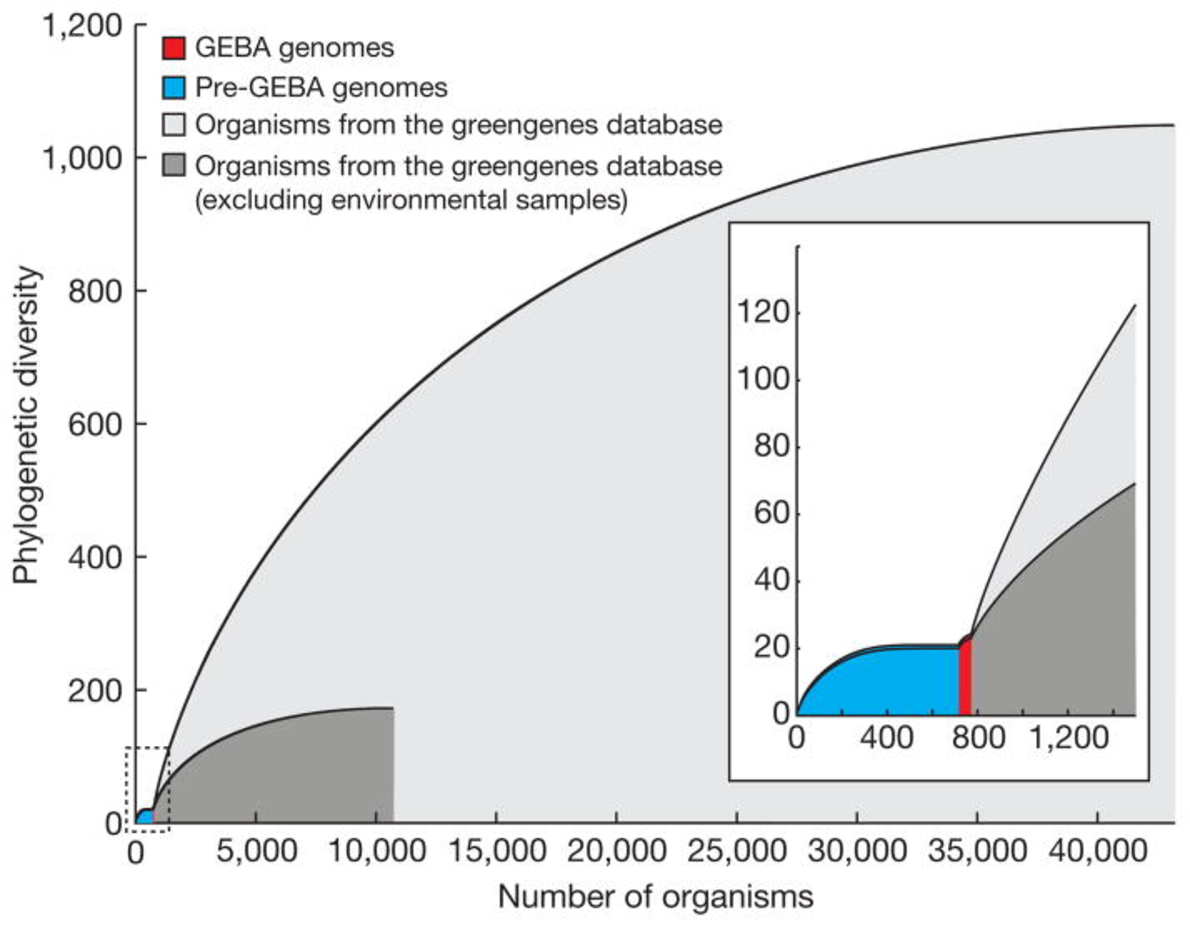
\includegraphics[width=100mm]{conc_figures/prok_diversity.pdf}
\caption[Plot of the diversity of \emph{Bacteria} and \emph{Archaea} from \citet{Wu2009}]{ Plot of the diversity of \emph{Bacteria} and \emph{Archaea} from \citet{Wu2009}. 
The diversity as shown by sequencing of 16S \acp{SSU} genes from the environment, from known organisms and from genomes is compared.
The inset shows the diversity encompassed from sequenced genomes before and after the Genomic Encyclopedia of \emph{Bacteria} and \emph{Archaea} (GEBA) sequencing project, which targets genomes for sequencing based on phylogenetic diverisity \cite{Wu2009}.
}
\label{fig:prok_diversity}

\end{figure}


\section{Concluding remarks}
%Molecular data can be continued to be mined! 
%Serves as a record for prosterity
%Metagenomics is not enough! There needs to be functional data, single cell data, biochemical data.

